\documentclass{article}
% ----- Preamble
\usepackage[utf8]{inputenc} % police encodee en latin1=iso8859-1=Windows Latin 1 %
\usepackage[french]{babel} % police fr %
\usepackage{hyperref} % pour les references %
\usepackage{amsmath} % pour les formules de maths %
\usepackage{amssymb} % pour les symboles maths %
\usepackage{amsthm} % pour la mise en forme des theoremes %
\usepackage{aeguill} % pour les guillemets et accents francais %
\usepackage{listings} % pour les listings de code %
\usepackage{helvet} % police helvetica %
\usepackage{graphicx}
\usepackage{dsfont}
\usepackage{subcaption}
\usepackage{caption}
% modification des dimensions de la page et de son centrage %
\topmargin 0.0cm
\oddsidemargin 0.1cm
\textwidth 16cm 
\textheight 22cm
\footskip 0.0cm

\title{Traitement d'Image et du Signal - TP6}
\author{Laurent Cetinsoy, Karim Kouki, Aris Tritas }
\date{\today}

\begin{document}
\maketitle


\section{Déconvolution par division et par filtre de Wiener}

On compare la déconvolution par division de la TFD et par filtrage de Wiener. On a d'abord déconvolé l'image par division de sa TFD avec différentes gaussiennes de variance $\sigma$. On a ensuite effectué le même traitement sur des images bruitées. Enfin on a déconvolé l'image bruitée à l'aide du filtre de Wiener.


\begin{figure}[h]
	\includegraphics[width=0.3\textwidth]{{deconvolution_sigma_3.5}.png}
	\includegraphics[width=0.3\textwidth]{deconvolution_sigma_4.png}
	\includegraphics[width=0.3\textwidth]{{deconvolution_sigma_4.5}.png}

  \caption{La variance de la gaussienne servant à déconvoluer est égale de gauche à droite, \\ $\sigma = 3.5, \;4,\; 4.5$ .}
\end{figure}

Pour des faibles valeurs de $\sigma$ la déconvolution par division de la TFD semble marcher. Néanmoins pour des plus grandes valeurs de $\sigma$ des artefacts apparaissent sur l'image (cf figure 1).

De plus la déconvolution par division est inopérente sur des images bruitées (cf figure 2).


\begin{figure}[h]
	\includegraphics[width=0.3\textwidth]{{deconvolution_sigma_3.5}.png}
	
\includegraphics[width=0.3\textwidth]{deconvolution_sigma_1_noise_0_01.png}
	\includegraphics[width=0.3\textwidth]{{deconvolution_wiener_sigma_g_3.5_noise_10_lambda_1}.png}

  \caption{A gauche (A) l'image sans bruit déconvoluée par division. Au milieu la même image bruitée $\sigma = 0.01 $ (B). A droite l'image bruitée déconvoluée par le filtre de Wiener (C). }
\end{figure}

Le filtre de Wiener quant à lui est robuste à l'ajout de bruit.

\section{Echange de phase}

Dans cette partie on s'intéresse à l'information portée par la phase et le module de la TFD d'une image. On a mélangé deux images en prenant le module de la TFD de l'une et la phase de la TFD de la seconde.

Dans un premier temps on a utilisé la phase de l'image de Lenna qu'on a mélangé avec le module de l'image de Barbara. Dans un second temps on à nouveau utilisé la phase de Lenna avec une image aléatoire générée par une Gaussienne. Enfin on a utilisé la phase de Lenna avec le module d'une image grise homogène: $I(i,j) = 0.5$.

\begin{figure}[h]
	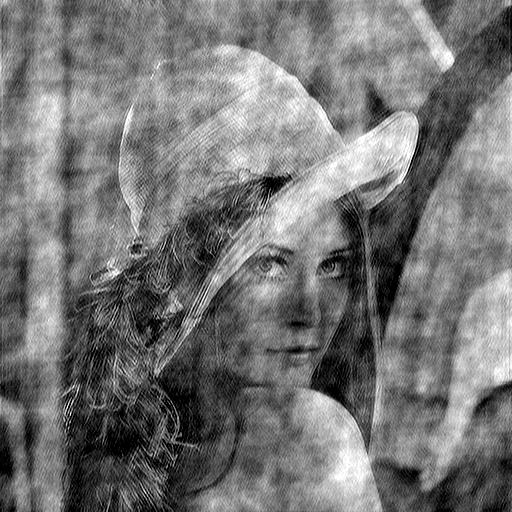
\includegraphics[width=0.3\textwidth]{phase_swapping.jpg}
	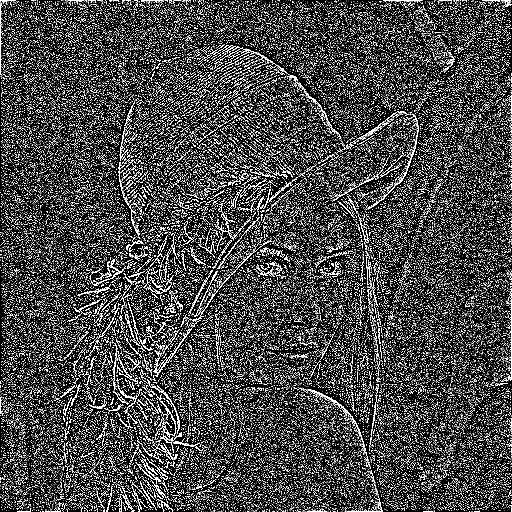
\includegraphics[width=0.3\textwidth]{phase_swapping_in_random.jpg}
		
\includegraphics[width=0.3\textwidth]{phase_swapping_in_grey_image.jpg}

  \caption{A gauche la phase de lena qui a été mélangée au module de barbara. Au milieu, la phase de lena projetée sur une image générée par une gaussienne. A droite la phase de Lena est exportée dans une image grise homogène.}
  
\end{figure}

On constate qu'une grande partie de l'information est portée par la phase. Inversement on voit que si on transfère le module de l'image de Lena dans Barbara, on voit bien Barbara.

Néanmoins la phase seule ne suffit pas (cf figure.2) : si on transporte la phase sur une image uniforme, l'image reste inchangée après transport de phase. 

On voit que le module ne porte que peu d'information mais a quand même besoin d'être présent. 

\newpage

\section{Ré-haussement des couleurs}


\begin{figure}[h]

	\includegraphics[width=0.3\textwidth]{edouart-manet-berthe-morisot.jpg}
	\includegraphics[width=0.3\textwidth]{edouart-manet-berthe-morisot-boosted.jpg}
	\includegraphics[width=0.3\textwidth]{edouart-manet-berthe-morisot-deboosted.jpg}
  \caption{A gauche image originale (Berthe Morisot de Manet). Au milieu, H augmenté de 150 \%. A droite diminué de 50 \%}
\end{figure}

On voit que le réhaussement de couleur accentue la coloration de l'image. Les parties noires de l'image ne sont pas impactée par le procédé. On peut supposer que les pixels blancs ne seraient pas impactés non plus. Inversement l'atténuation de H, l'image "décolore" l'image en lui donnant l'apparence d'une image en niveau de gris.

\newpage

\section{Changement de contraste}

\subsection*{Question 1}

Dans cette partie on s'intéresse à un réhaussement de contraste par transformation affine :

$$I'(i,j) = \frac{1}{min-max} * (I(i,j) - min)$$

\begin{figure}[h]

	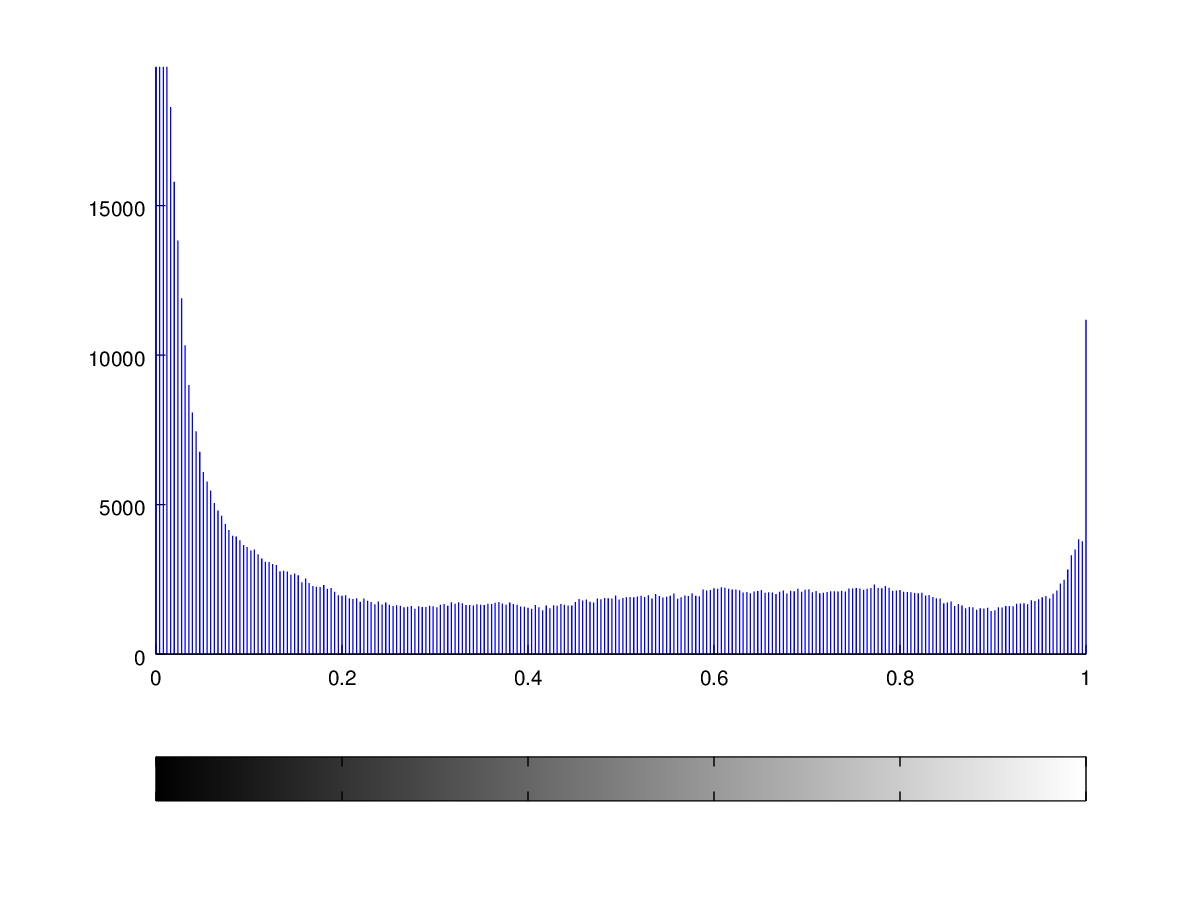
\includegraphics[width=0.5\textwidth]{hist_orig.png}
	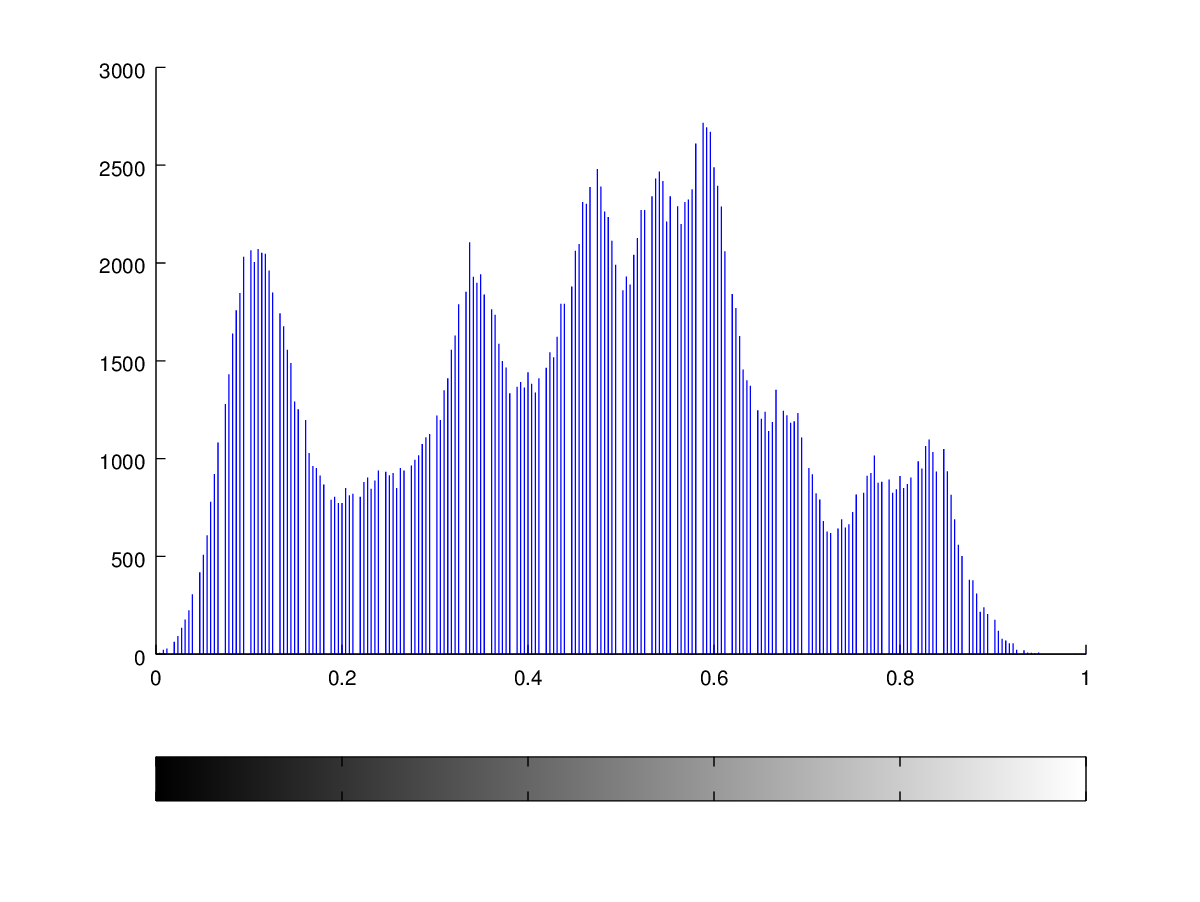
\includegraphics[width=0.5\textwidth]{hist_scaled.png}

\centering
	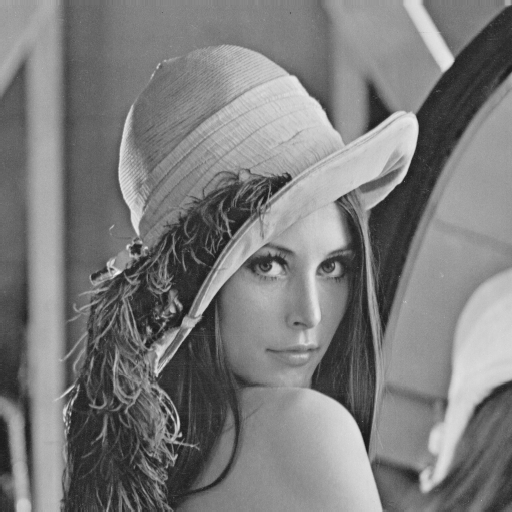
\includegraphics[scale=0.4]{lena.png}
	\includegraphics[scale=0.4]{lena_hist_scaled.png}
		
	\caption{A gauche l'image et l'histogramme originaux. A droite après changement de contraste affine}
	
\end{figure}

On constate que l'image de droite a un contraste renforcé. On voit que l'histogramme est étiré : les écarts entre les niveaux de gris sont uniformisés.  

\subsection*{Question 2}

Dans le cas où il existe dans l'image un pixel qui est nul et un pixel d'intensité maximal (1). Alors la transformation affine n'a aucun effet : $\min I(i,j) = 0 \;\;\; \max I(i,j) = 1$
	
$$I'(i,j) = \frac{1}{\min-\max} * (I(i,j) -\min) = I(i,j)$$


\begin{figure}[h]
		
	\caption{A gauche l'image et l'histogramme originaux. A droite après changement de contraste affine}
	
\end{figure}


Une solution est de remplacer $\min I(i,j)$ par $\min I(i,j) + \epsilon$ et $\max$ par $\max I(i,j)$ par $\max I(i,j) - \epsilon$.
Il est aussi possible de remplacer uniquement les pixels de valeurs 0 et 1 par $\epsilon$ et $1-\epsilon$ respectivement.


\section{Filtre médian}
	Dans le cas où du bruit de type salt'n'pepper entâche le signal de l'image que l'on souhaite traiter, le filtre médian se révèle particulièrement efficace. Le filtre est un processus itératif qui lisse l'image en définissant une fenêtre carrée autour de chaque pixel,  calcule la valeur médiane de l'intensité des pixels de la fenêtre et assigne celle-ci au pixel courant.
	
\begin{figure}[h]

	\includegraphics[width=0.5\textwidth]{median_noisy.png}
	\includegraphics[width=0.5\textwidth]{median_denoised.png}
	\caption{A gauche l'image bruitée donnée en entrée au filtre médian et à droite le résultat du débruitage.}
	
\end{figure}
\newpage
\section{Travail écrit}

\subsection{Convolution}
On rapelle l'expression de la transformée de Fourier:
$ \hat{f}(\xi) = \int_\mathbb{R} f(x) e^{-ix\xi} \:\mathrm{d}x$

On s'intéresse à la fonction: $ f_K : \mathbb{R} \ni x \rightarrow \frac{\mathds{1}_{[0, K]}(x)}{K}, K \in \mathbb{R}_+^* $

\begin{equation*}\begin{split}
\hat{f_K}(\xi) 
&= \int_\mathbb{R} \frac{\mathds{1}_{[0, K]}(x)}{K} e^{-ix\xi} \:\mathrm{d}x \;=\; \int_0^{K} \frac{1}{K}e^{-ix\xi}\:\mathrm{d} x \\
&= -\frac{1}{i \xi K} e^{\frac{-i \xi K}{2}}\bigg [ e^{\frac{-i \xi K}{2}} - e^{\frac{i \xi K}{2}} \bigg] \\
&= \frac{2}{\xi K} e^{\frac{-i \xi K}{2}} \sin(\frac{\xi K}{2\pi})\\
&= e^{\frac{-i \xi K}{2}} \text{sinc}(\frac{\xi K}{2\pi})
\end{split}\end{equation*}

\subsection{Flou de bougé}
\begin{enumerate}
\item Si K est strictement positif, le dénominateur de la transformée de Fourier calculée précédemment ne s'annule pas. La convolution par $f_K$ est donc inversible.

On calcule ainsi la convolution de $f = u$ et $g =f_{v \Delta t} \times \Delta t $. Ainsi,
\begin{equation*}\begin{split}
(f * g)(x) = \int_\mathbb{R} u(x-z)\frac{\mathds{1}_{[0, v \Delta t]}(x)}{v \Delta t} \Delta t \:\mathrm{d}z \; = \;   \int_{0}^{v \Delta t} \frac{u(x-z)}{v} \:\mathrm{d}z
\end{split}\end{equation*}

En posant le changement de variable affine: $ z=v t $, on obtient les bonnes bornes d'intégration et la formule souhaitée:
$$(f * g)(x) = \int_{0}^{\Delta t} u(x-vt)\:\mathrm{d}t$$
\item Le flou perçu dépend de $v$:

\begin{itemize}
\item Si pendant le temps $\Delta t$, la distance $v \Delta t$ parcourue par l'objet observé est inférieure à la résolution du capteur, l'image observée ne sera pas forcément perçue plus floue.
\item Inversement, si pendant le temps $\Delta t$, la distance $v \Delta t$ est suffisamment importante, plus les zones réceptrices du capteur vont recevoir des photons d'un objet qui a bougé d'autant plus avec l'augmentation de $\Delta t$. Dans ce cas de figure, l'objet est perçu plus flou.
\end{itemize}

\item Pour simuler un flou de bougé, on peut utiliser l'algorithme:
\begin{itemize}
\item On choisit $v \; et \; \Delta t$ 
\item On calcule la TFD de l'image et celle de la fonction porte
\item On réalise le produit de convolution par multiplication des TFD de l'image et de la fonction porte
\item Finalement on prend la TFD inverse afin de pouvoir visualiser l'image.
\end{itemize}

\end{enumerate}
\end{document}